\documentclass{article}
\usepackage{spconf,amsmath,graphicx}
\usepackage{float, adjustbox}
\graphicspath{ {images/} }

% Example definitions.
% --------------------
\def\x{{\mathbf x}}
\def\L{{\cal L}}

\title{Fundamentals Aided Stock Forecasting with Long Short Term Memory Neural Networks}

\name{Evan Kozliner, Debanjan Nandi, Isaac Goldthwaite, Aaditya Gavandalkar}
\address{Computer Science and Engineering, The Ohio State University}
\begin{document}
%\ninept
%
\maketitle
%
\begin{abstract}
We build a Long Short Term Memory (LSTM) neural network model to evaluate how such a network performs when regressing stock price data and to examine the impact of fundamentals data on the LSTM. LSTM models are often used as predictive models for temporal data due to their ability to retain information about long term pattern in data. There have been some attempts to utilize LSTMs for time series predictions like stock pricing, currency pricing, and stock volatility\cite{maknickienė_rutkauskas_maknickas_2011}, but it seems that few have examined whether or not financial fundamentals such as balance sheet data can impact their accuracy. The results suggest that the LSTM does not effectively utilize the fundamentals information we provided.
\end{abstract}
%
\begin{keywords}
Long Short Term Memory Neural Networks, Stock Forecasting, Recurrent Neural Network
\end{keywords}
%
\section{Introduction}
\label{sec:intro}

To analyse the price of stocks generally one of two methods are employed: technical or fundamentals analysis. Fundamentals analysis attempts to measure the intrinsic value of a stock by studying quarterly metrics such as a company’s assets and liabilities, or macro trends like the performance of a whole sector of the economy.  Technical analysis generally does not incorporate these figures and instead relies mostly on figures like a security’s price and volume traded, typically represented as a time series. 

The accuracy of regression techniques to predict future stock prices is paramount in technical analysis because it is used to compute a stock's future value and volatility. The volatility and return potential of a stock relative to another dictates which stock is a better purchase.

LSTM models are type of recurrent neural networks (RNNs) that can handle temporal data and be used to make time series predictions. LSTM models are of a particular interest in the domain of time series prediction because they have the capability to pick up patterns in data spanning long periods of time, unlike traditional RNNs, which suffer from the vanishing gradient problem when picking up long term patterns and other temporal models. Neural networks in general have the capacity to pick up complex relationships between input data, so there is some chance that that given the right data the LSTM could pick up difficult-to-spot but significant relationships between fundamentals data and stock prices.  

Any overview of stock price prediction would be incomplete without mentioning the Efficient Market Hypothesis (EMH)\cite{malkiel_2003} and its implications on the feasibility of trading systems. EMH argues that it is impossible to “beat the market” because the stock price is always representative of its fair value. If EMH is correct, it would nullify the point of doing stock analysis at all and suggest that it would be better to purchase index funds. 

Another potential problem for the incorporation of fundamentals data in stock price analysis is the risk that stock prices actually have little to do with the intrinsic value of a company. Behavioural economics suggests that investors are subject to  cognitive biases when investing in a company. These biases can cause investors to pick growth stocks that are more frequently reported on over companies with good fundamentals. This behaviour inflates the price of “hot stocks” and leaves many companies unnoticed. The effect of human psychology could be good or bad for trading systems depending on if the trading systems are able to pick up on human patterns of undervalues and overvaluing. 

\section{Data Extraction}
\label{sec:data_extraction}

Historical stock price data is not frequently provided minute-by-minute, instead it is provided daily and only includes the opening price of the stock, the closing price, the highest price the stock reached, and the lowest price. This data is readily available online, we used the python backtesting framework ‘bt’ to obtain it. 

The data prior to adding fundamentals was indexed by day and looked like the following:
\begin{table}[H]
\centering
\begin{tabular}{|l|l|l|l|l|}
\hline
 & Open & High & Low & Close \\ \hline
2011-01-03 & 181.36 & 186.00 & 181.21 & 184.22\\ \hline
2011-01-04 & 186.14 & 187.69 & 183.77 & 185.00 \\ \hline
2011-01-05 & 184.10 & 187.44 & 184.07 & 187.41\\ \hline
\end{tabular}
\caption{Stock data before adding fundamentals information}
\label{my-label}
\end{table}

Fundamentals data is can be difficult to obtain because it needs scraped off 10-K or 10-Q (yearly or quarterly) reports. All of these reports are available through an FTP server provided by the SEA, written in a standard format known XBRL. An open source tool called ScraXBRL can extract the data from these reports into a tree structure, however manual tree search algorithms needed to be written manually to extract specific values from the report. Scripts also needed to be written to properly join fundamentals data (which only comes quarterly) with daily stock prices. 

Out of the large amount of fundamentals data only “Cash and Cash Equivalents”, “Net Assets”, and “Net Liabilities” were selected as features for the LSTM. These features were selected because they are some of the simplest indicators of a company's financial success. Common financial ratios such as the P/E ratio would be a logical next step, however we only wanted to examine some of the most bare-bones fundamentals for our analysis. 

After the addition of the fundamentals data our input vectors included below features in addition to previously mentioned stock features like this (note the fundamentals data is repeated because the same fundamentals apply for the whole quarter):
\begin{table}[H]
\centering
\begin{adjustbox}{width=0.5\textwidth}
\small
\begin{tabular}{|l|l|l|l|l|l|l|l|}
\hline
 & Open & High & Low & Close  & Cash & Assets & Liabilities \\ \hline
2011-01-03 & 181.36 & 186.00 & 181.21 & 184.22 & 3.77e+09 & 1.879e+10 & 1.037e+10 \\ \hline
2011-01-04 & 186.14 & 187.69 & 183.77 & 185.00 & 3.77e+09 & 1.879e+10 & 1.037e+10 \\ \hline
2011-01-05 & 184.10 & 187.44 & 184.07 & 187.41 & 3.77e+09 & 1.879e+10 & 1.037e+10 \\ \hline
\end{tabular}
\end{adjustbox}
\caption{Additional fundamentals data added to input vector}
\end{table}

Our goal was to predict the “Close” column of each day using the other pieces of data in the columns. We also decided to include a “previous day close price” feature, which boosted accuracy. 

To demonstrate the correlation between the closing price and fundamentals data we measured the Pearson correlation between the Cash, Assets, and Liabilities columns and the closing prices for Amazon (ticker AMZN):
\begin{table}[H]
\centering
\begin{adjustbox}{width=0.3\textwidth}
\small
\begin{tabular}{|l|l|}
\hline
Fundamental & Pearson Correlation \\ \hline
Assets      & .9411               \\ \hline
Liabilities & .9017               \\ \hline
Cash        & .8562               \\ \hline
\end{tabular}
\end{adjustbox}
\caption{Pearson correlation for stock fundamentals}
\label{my-label}
\end{table}
These were measured using the scipy.stats library. All of the values have strong positive correlations with the closing price, which suggests that the neural net might be able to find some edge utilizing them alongside the opening price data. 

\section{Linear Regression Baseline}
\label{sec:linear_regression}
A common approach used when predicting stock market data is to model past data with a series of linear regressions to predict future results. As a baseline to compare our prediction model, we used a linear regression model which trained on past open values versus same-day close values. This model was then used to predict future close values given the same-day open values as well as previous day close values in our data’s test set. Below are the results we found:

\begin{figure}[H]
\centering
\includegraphics[width=0.5\textwidth]{basic_regression_RMSE_with_prev_day}
\caption{Result of linear regression using same day open and previous day close values for Amazon (NASDAQ: AMZN)}
\label{fig:linear_withoutfunda}
\end{figure}

Results produced by above mentioned linear regression model wihtout using fundamentals data had RMSE of 8.23 on test dataset and 4.08 on training dataset. We also ran tests on a linear regression model that took into account the fundamentals data , training on not only the opening and closing values, but also the cash and cash equivalents at carrying value, assets, and current liabilities. 

\begin{figure}[H]
\centering
\includegraphics[width=0.5\textwidth]{linear_only_open_and_close}
\caption{Result of linear regression using same day open, previous day close values and fundamentals for Amazon (NASDAQ: AMZN)}
\label{fig:linear_withfunda}
\end{figure}

Results produced by linear regression model while using fundamentals had RMSE of 8.729 on test dataset and 4.0739 on training dataset. Overall, the linear regression model using fundamentals data did not show significant improvement on the over the regression model that did not utilize the fundamentals data.

\section{Long short-term memory (LSTM)}
\label{sec:lstm}
\begin{figure}[h]
\centering
\includegraphics[width=0.5\textwidth]{LSTMarch}
\caption{Illustrates a single LSTM memory cell}
\label{fig:lstmcell}
\end{figure}

Long Short Term Memory (LSTM) architecture\cite{hochreiter_schmidhuber_1997} uses special purpose-built memory cells to store information and is better at finding and exploiting long range dependencies in the data. Fig\ref{fig:lstmcell} illustrates a single LSTM memory cell. The memory cells, with self-connections storing the temporal state of the network, are key to the “memory” of the to the LSTM. Each LSTM block also contains an input gate, an output gate, and a forget gate. The input gate controls the input flow of data and determines by how much we should update each memory cell value. The forget gate determines which values of the cell state should be retained and which values to be forgotten. The output gate controls the output flow of data and determines what parts of the cell state we are going to output.

A LSTM calculates the network unit activations using the following equations iteratively from t = 1 to T:

\begin{equation}
ft  = \sigma ( Wf.[ht-1, xt] + bf)
\end{equation}
\begin{equation}
It  = \sigma ( Wi.[ht-1, xt] + bi)
\end{equation}
\begin{equation}
ot  = \sigma ( Wo.[ht-1, xt] + bo)
\end{equation}
\begin{equation}
ct = ft \circ ct-1  +  it \circ\sigma ( Wc.[ht-1, xt] + bc)
\end{equation}
\begin{equation}
ht = ot \circ tanh(ct)
\end{equation}

Where $\circ$ denotes the Hadamard product, $\sigma$ is the sigmoid function, i, f, o and c are respectively the input gate, forget gate, output gate and cell activation vectors, all of which are of the same same size as the hidden vector h. W and b represent the corresponding weight matrices and bias vectors for the respective gates.

\section{Implementation}
\label{sec:implementation}

We used an embedding dimension of 64 for all the attributes of the feature vectors before using them as input to the LSTM. We used a fixed hidden state dimension of 1024 for all the LSTM modes. Additionally we use a dense hidden layer of a single neuron on top of the 2 hidden LSTM layers to determine the closing price. We used a learning rate of 0.001 and an Adam Optimizer minimizing the RMS Error for training the model for 100 epochs. The model was trained on a single GPU with Tensorflow implementation. We used a sliding window of 20 sequences. The batchsize was maintained at 128 sequences per batch

\textbf{MENTION RANDOM SELECTION OF SEQUENCES and WHY NOT TO USE LOOKBACK}

\section{Evaluation}
\label{sec:implementation}

\subsection{Evaluating effects of fundamentals data on stock forecasting}
\label{ssec:lstm_fundamentals_data}

We ran tests to predict future close values given the same-day open values as well as previous day close value in our data’s test set both with as well as without any fundamentals data. Below are the results of these two configuration:

\begin{figure}[h]
\centering
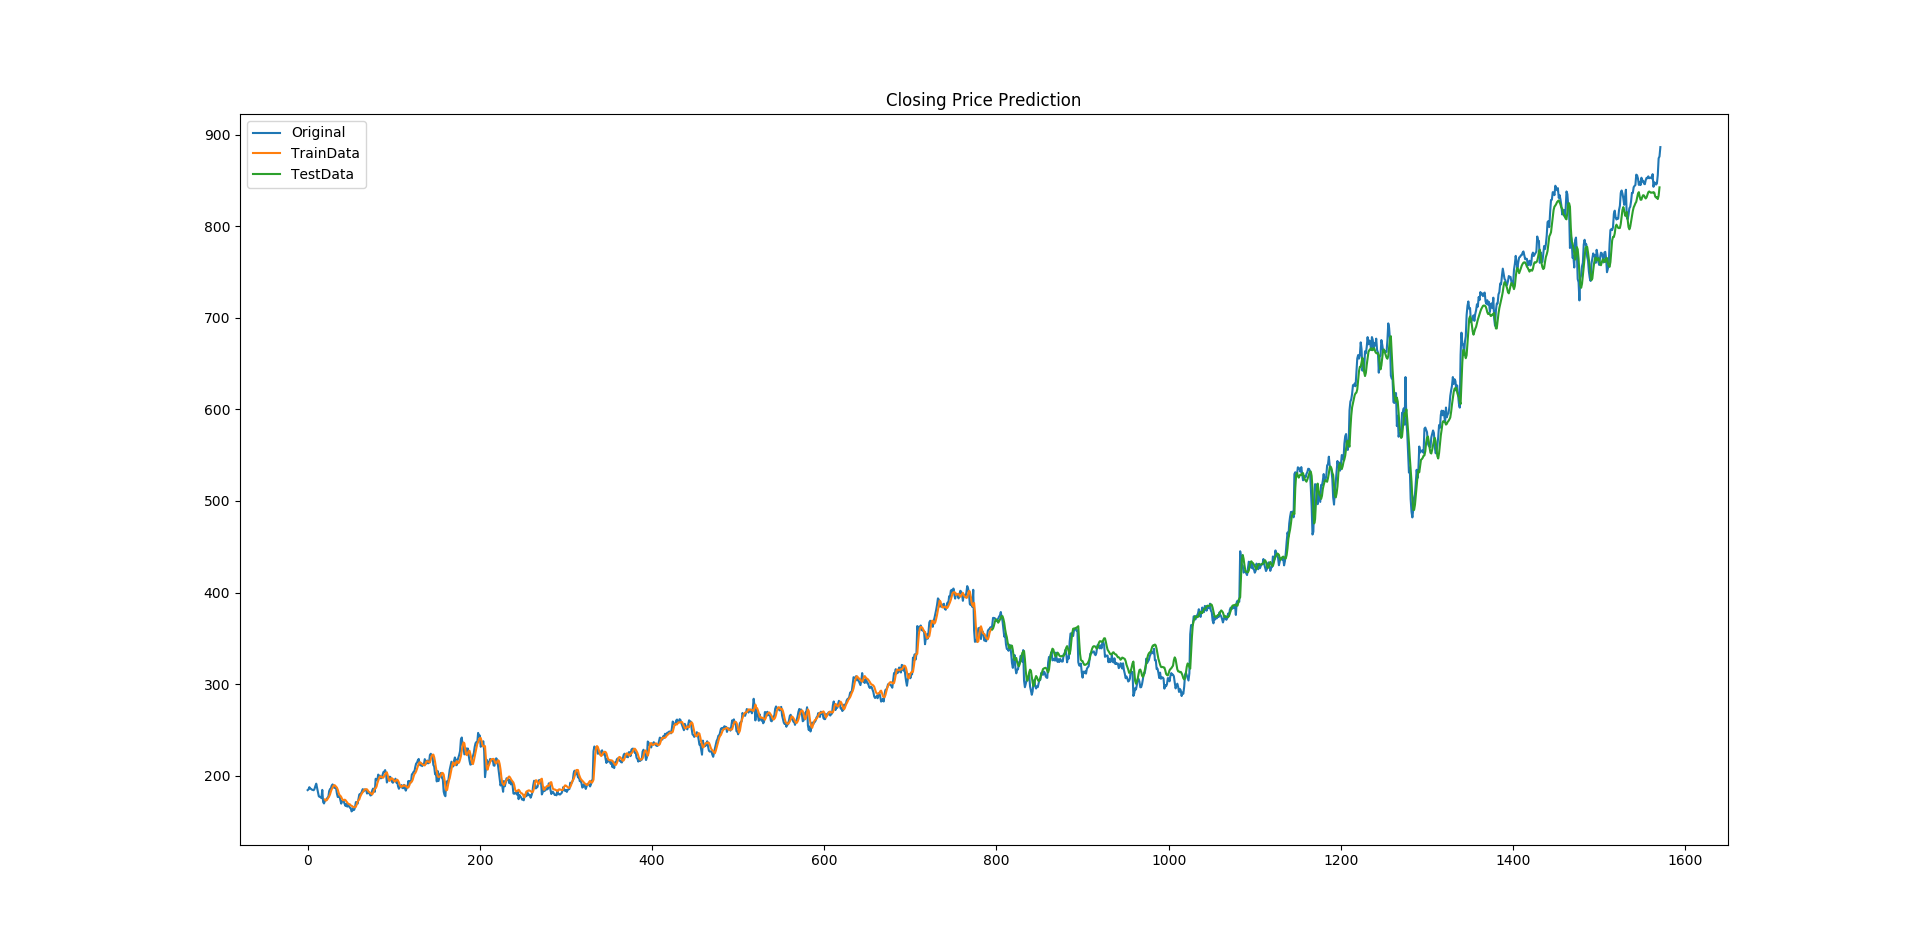
\includegraphics[width=0.5\textwidth]{amazon_incl_fundamentals}
\caption{Amazon(NASDAQ: AMZN) stock price prediction when using fundamentals data}
\label{fig:amazon_with_funda}
\end{figure}

\begin{figure}[h]
\centering
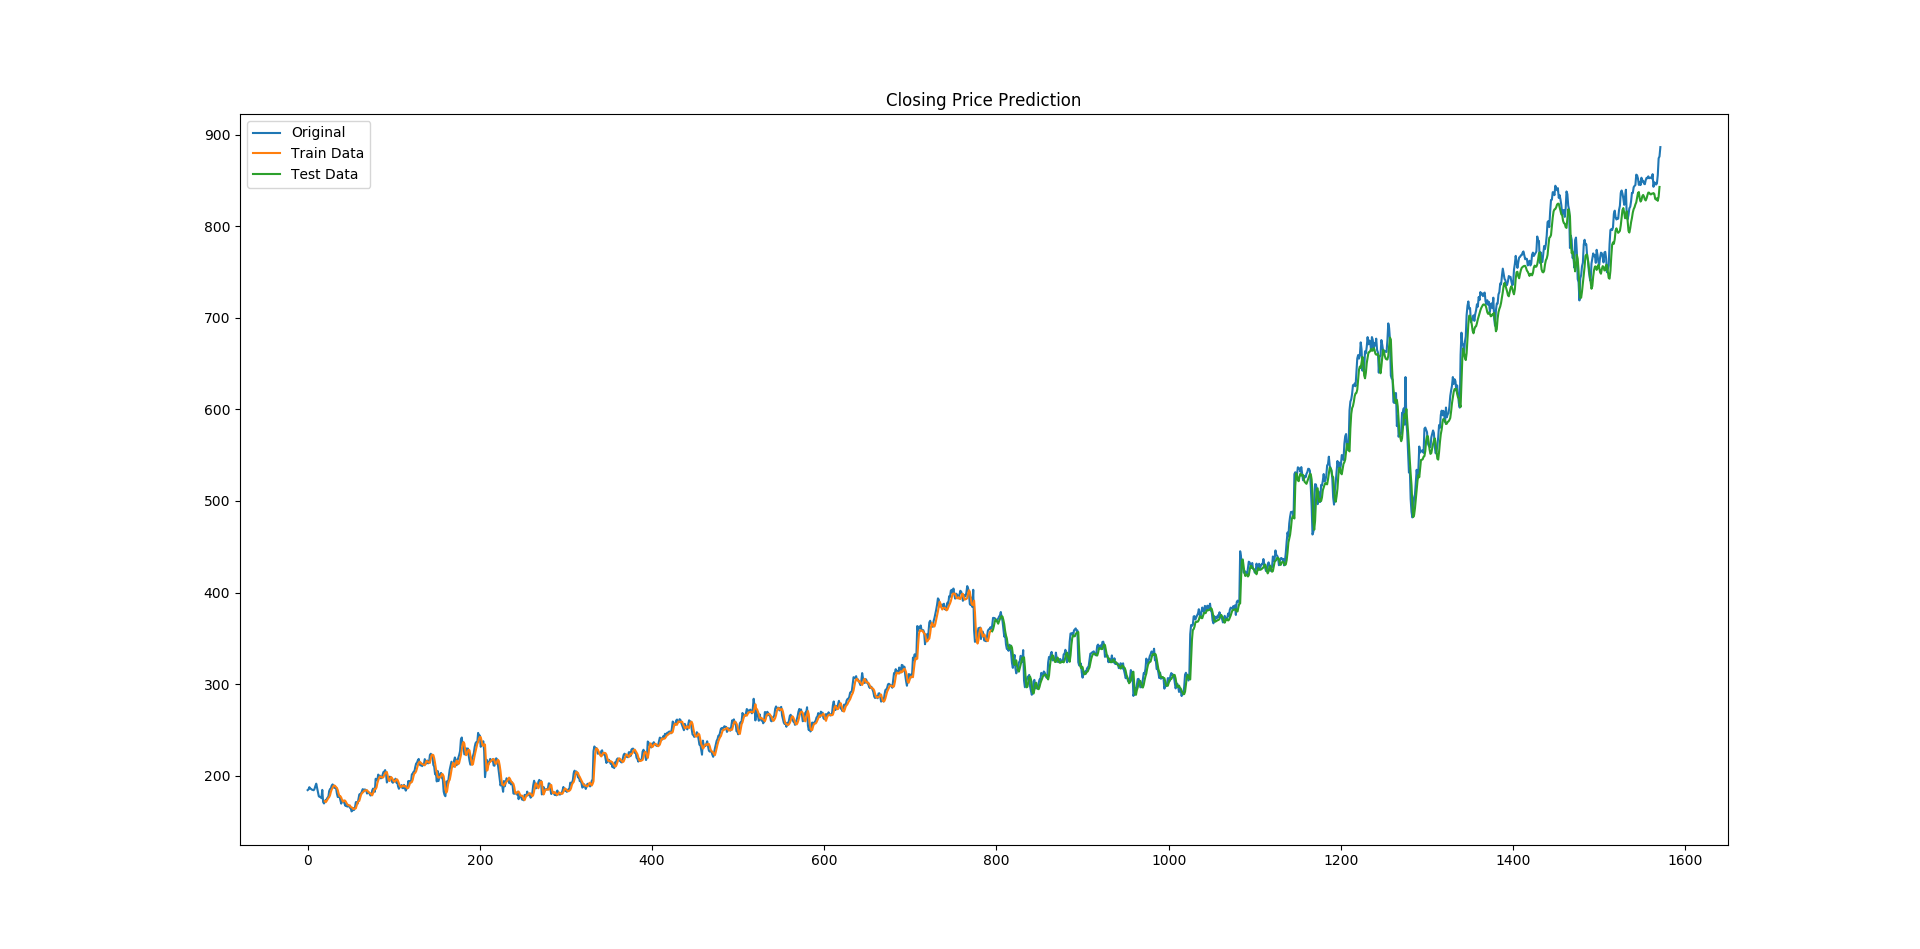
\includegraphics[width=0.5\textwidth]{amazon_without_fundamentals}
\caption{Amazon(NASDAQ: AMZN) stock price prediction without using fundamentals data}
\label{fig:amazon_without_funda}
\end{figure}

Overall, the fundamentals data did not have a significant effect on the accuracy of the LSTM model. Below are the MSE values that we found in the above two cases:
\begin{table}[H]
\centering
\label{evaluation_mse_amazon}
\begin{tabular}{|l|l|}
\hline
                          & MSE (test dataset)          \\ \hline
Without fundamentals data & 12.0814 \\ \hline
With fundamentals data    & 11.4807 \\ \hline
\end{tabular}
\caption{MSE values found while forecasting with and without fundamentals data included}
\end{table}
 
\subsection{Evaluating feautre set for predicting closing price after stock splits}
\label{sssec:predicting_stock_splits}

Predicting closing price of any stock immediately after its split is another challenge one could face during the process. Most likely the fundamentals data is going to remain same for before and after split dates considering the dates belong to same quarter with a high probability. Availability of features and choice of features used for prediction affect how accurate the prediction will be in this case. For example consider Netflix. Netflix (NASDAQ: NFLX) stock went under 7-for-1 stock split on 15th July 2015.
\begin{table}[H]
\centering
\label{my-label}
\begin{adjustbox}{width=0.5\textwidth}
\small
\begin{tabular}{|l|l|l|l|l|}
\hline
Date & Actual price & \begin{tabular}[c]{@{}l@{}}Prediction\\ (FV + \\Prev day close)\end{tabular} & \begin{tabular}[c]{@{}l@{}}Prediction\\ (FV + \\Same day open)\end{tabular} & \begin{tabular}[c]{@{}l@{}}Prediction\\ (FV + \\Prev day close + \\Same day open)\end{tabular} \\ \hline
2015-07-14 & 702.600006 & result\_here & result\_here & result\_here \\ \hline
2015-07-15 & 98.129997 & result\_here & result\_here & result\_here \\ \hline
\end{tabular}
\end{adjustbox}
\caption{Results for different feature vector configurations (FV = Fundamental data vector)}
\end{table}
As expected the available quarterly fundamentals data remain same for both of these dates and don’t contribute much towards making the correct prediction. Whereas other features like same day open price and previous day close price does affect the prediction which are summarised in table above. As expected, not using same day open price leads to incorrect prediction whereas using helps making a prediction closer to actual price.

\begin{figure}[H]
\centering
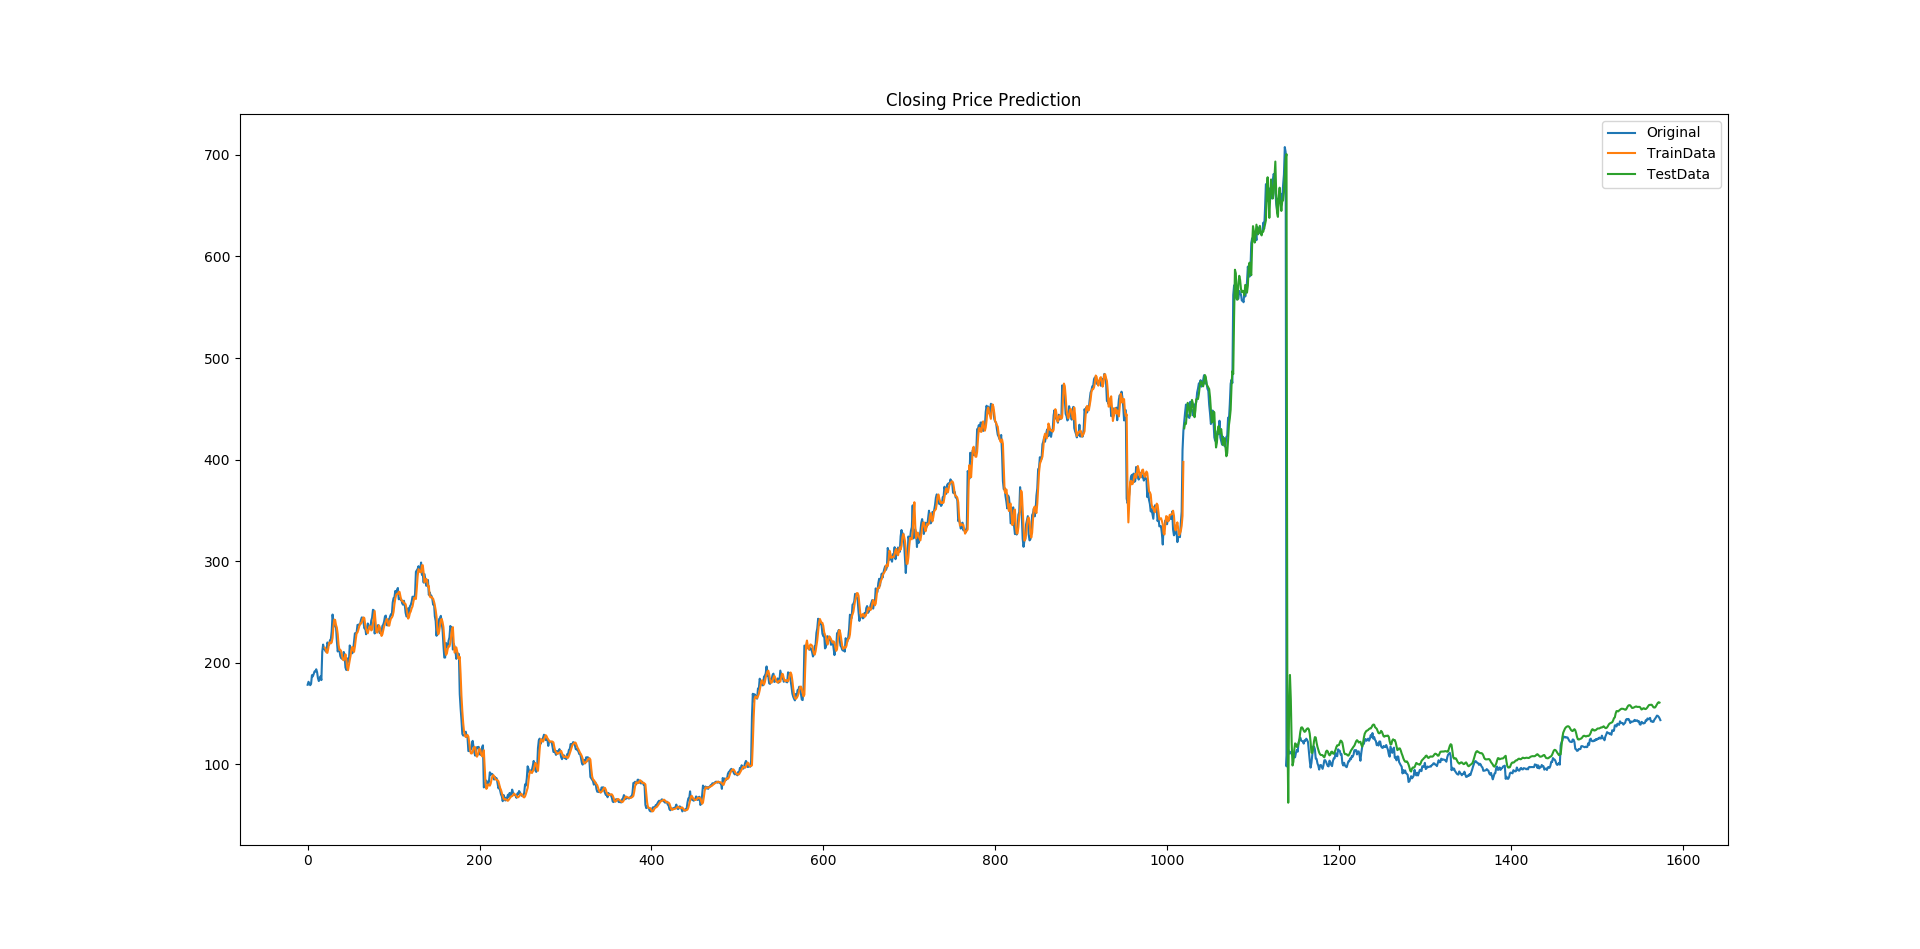
\includegraphics[width=0.4\textwidth]{netflix_incl_funda}
\caption{Netflix(NASDAQ: NFLX) stock price prediction}
\label{fig:netflix_with_funda}
\end{figure}

\section{Conclusion}
\label{sec:conclusion}


\nocite{maknickienė_maknickas}
\nocite{ding_zhang_liu_duan_2015}
\bibliographystyle{IEEEbib}
\bibliography{strings,refs}
\end{document}